\section{Proximal-escape radii under affine constraints}
\label{sec:escape}

After the SDG identifies a KKT candidate, proximal escape turns to a second
safe proximal construction: the hard-constrained proximal map of
\(f+\ind_{\Cset}\).  Its outputs are feasible by construction, unlike the
Lagrangian proximal comparison defining the SDG.  The escape radius measures
the center-perturbation scale at which proximal polishing produces a strictly
lower objective value.

\subsection{Escape radius and its classification}
\label{subsec:escape-profile}

Throughout this section, \(x\in\Cset\cap\operatorname{dom} f\), \(\lambda>0\),
\(\lambda\rho<1\), and \(P_\lambda^{\Cset}\) denotes the unique constrained
proximal map in \cref{eq:cprox}.  Center perturbations belong to
\(\Tspace=\ker A\), so \(x+d\) satisfies the affine equality but need not
belong to \(\operatorname{dom}f\).  For example, a center may lie outside
an implicit box, whereas its proximal output must belong to
\(\Cset\cap\operatorname{dom}f\).
For \(\delta\ge0\), define the best polished value
\begin{equation}
  \Phi_{\lambda,\delta}(x)
  :=
  \inf_{\substack{d\in\Tspace\\\norm d\le\delta}}
  f\!\left(P_\lambda^{\Cset}(x+d)\right)
  \label{eq:escape-profile}
\end{equation}
and its associated decrease
\begin{equation}
  \Rprox_{\lambda,\delta}(x)
  :=
  f(x)-\Phi_{\lambda,\delta}(x).
  \label{eq:prox-drop}
\end{equation}
The quantity \(\Rprox_{\lambda,\delta}(x)\) is nonnegative and nondecreasing
in \(\delta\).  It is nonnegative because the unperturbed center is
admissible and proximal optimality gives
\(f(P_\lambda^{\Cset}(x))\le f(x)\); it is monotone because the set of
admissible centers grows with the radius.

\begin{definition}[Proximal-escape radius]
  \label{def:escape-radius}
  The ideal proximal-escape radius of \(x\) is
  \begin{equation}
    r_{\lambda}^{\mathrm{esc}}(x)
    :=
    \inf\{\delta>0:
             \Rprox_{\lambda,\delta}(x)>0\},
    \label{eq:escape-radius}
  \end{equation}
  with the convention \(\inf\varnothing=+\infty\).
\end{definition}

When \(r_{\lambda}^{\mathrm{esc}}(x)=0\), arbitrarily small center
perturbations yield a lower polished value.  A finite positive radius gives a
positive neighborhood \(0<\delta<r_{\lambda}^{\mathrm{esc}}(x)\) on which the
polished decrease is zero, followed by positive decrease at every larger
radius.  An infinite radius means that no feasible center produces a lower
proximal output.

Monotonicity makes the threshold interpretation precise.  If
\(r=r_{\lambda}^{\mathrm{esc}}(x)\), then
\(\Rprox_{\lambda,\delta}(x)=0\) for every \(0<\delta<r\).  If \(r<+\infty\),
then \(\Rprox_{\lambda,\delta}(x)>0\) for every \(\delta>r\).  No conclusion
about the boundary follows from monotonicity alone, but the standing
assumptions provide the missing regularity.  Indeed,
\[
  f(P_\lambda^{\Cset}(z))
  =
  \Moreau_\lambda^{\Cset}(z)
  -\frac{1}{2\lambda}\norm{P_\lambda^{\Cset}(z)-z}^{2}
\]
is continuous because the envelope is continuous and
\(P_\lambda^{\Cset}\) is Lipschitz.  Hence, for every finite \(\delta\), both
this function and the envelope attain their minima on the compact set
\(D_\delta:=\Tspace\cap B_\delta(0)\).  To justify continuity of the outer
value, write
\[
  h(d):=f(P_\lambda^{\Cset}(x+d)),
  \qquad
  v(\delta):=\min_{d\in D_\delta}h(d).
\]
If \(\delta_k\to\delta>0\), let \(d^\star\) minimize \(h\) on
\(D_\delta\) and set
\(d_k=\min\{1,\delta_k/\delta\}d^\star\).  Then
\(d_k\in D_{\delta_k}\), \(d_k\to d^\star\), and
\(\limsup_kv(\delta_k)\le v(\delta)\).  Conversely, choose minimizers in
\(D_{\delta_k}\) along a subsequence realizing the lower limit.  Compactness
gives a further subsequence converging to some \(\bar d\in D_\delta\), and
continuity of \(h\) gives
\(\liminf_kv(\delta_k)=h(\bar d)\ge v(\delta)\).  At \(\delta=0\), every
\(d_k\in D_{\delta_k}\) converges to zero.  Hence \(v\) is continuous on
\([0,+\infty)\); the same argument applies to the envelope outer value.
It follows that
\[
  0<r_{\lambda}^{\mathrm{esc}}(x)<+\infty
  \quad\Longrightarrow\quad
  \Rprox_{\lambda,r_{\lambda}^{\mathrm{esc}}(x)}(x)=0.
\]
When the radius is zero, the boundary value
\(\Rprox_{\lambda,0}(x)=f(x)-f(P_\lambda^{\Cset}(x))\) can instead be zero or
positive; it is zero whenever \(x\) is a proximal fixed point, as is the case
for the KKT candidates considered below.

The classification begins with a basic consequence of proximal optimality.
For every feasible center \(z\in\Cset\), setting
\(p=P_\lambda^{\Cset}(z)\) and using \(u=z\) as a competitor gives
\begin{equation}
  f(p)+\frac{1}{2\lambda}\norm{p-z}^{2}
  \le f(z).
  \label{eq:prox-polishing}
\end{equation}
Inequality~\eqref{eq:prox-polishing} shows that every direct feasible decrease
yields at least as large a polished decrease.  Define accordingly the direct
feasible decrease
\begin{equation}
  \mathcal{S}_\delta(x)
  :=
  f(x)
  -\inf_{\substack{u\in\Cset\\\norm{u-x}\le\delta}}f(u).
  \label{eq:direct-drop}
\end{equation}
For any feasible \(u=x+d\) in the radius-\(\delta\) ball,
\cref{eq:prox-polishing} gives
\(f(P_\lambda^{\Cset}(x+d))\le f(u)\).  Taking infima yields
\begin{equation}
  \Rprox_{\lambda,\delta}(x)\ge\mathcal{S}_\delta(x).
  \label{eq:prox-dominates-direct}
\end{equation}

The positive-radius statement also requires stability of the safe proximal
map.  By \Cref{lem:safe-constrained-prox}, its Lipschitz constant is at most
\((1-\lambda\rho)^{-1}\), the relevant weakly convex stability bound.

\begin{theorem}[Trichotomy for the ideal escape radius]
  \label{thm:radius-classification}
  Let \(f+\ind_{\Cset}\) be proper, lower semicontinuous, and
  \(\rho\)-weakly convex, and let \(\lambda>0\) with \(\lambda\rho<1\).  For a feasible point
  \(x\in\operatorname{dom} f\), exactly one of the following cases holds.
  \begin{enumerate}[label=(\roman*)]
    \item \(x\) is a global minimizer of \(f\) on \(\Cset\), and
          \(r_{\lambda}^{\mathrm{esc}}(x)=+\infty\).
    \item \(x\) is a nonglobal local minimizer of \(f\) on \(\Cset\), and
          \(0<r_{\lambda}^{\mathrm{esc}}(x)<+\infty\).  More precisely, if
          \(r_0>0\) satisfies
          \[
            f(u)\ge f(x)
            \qquad
            \text{for all }u\in\Cset\cap B_{r_0}(x),
          \]
          then
          \begin{equation}
            r_{\lambda}^{\mathrm{esc}}(x)
            \ge(1-\lambda\rho)r_0.
            \label{eq:escape-radius-lower}
          \end{equation}
    \item \(x\) is not a local minimizer of \(f\) on \(\Cset\), and
          \(r_{\lambda}^{\mathrm{esc}}(x)=0\).
  \end{enumerate}
  Equivalently, the three possible radius types \(+\infty\), \((0,+\infty)\),
  and \(0\) characterize, respectively, the three classes above.
\end{theorem}

\begin{proof}
  If \(x\) is globally minimizing, every proximal output is feasible and has
  objective value at least \(f(x)\).  The unperturbed center has proximal
  point \(x\), so \(\Rprox_{\lambda,\delta}(x)=0\) for every \(\delta\).
  Conversely, if a feasible \(z\) satisfies \(f(z)<f(x)\), then
  \cref{eq:prox-polishing} gives
  \(f(P_\lambda^{\Cset}(z))\le f(z)<f(x)\).  Taking
  \(\delta\ge\norm{z-x}\) proves that the escape radius is finite.  Hence the
  infinite-radius case is equivalent to global minimality.

  If \(x\) is not locally minimizing, every positive-radius feasible ball
  contains a point with smaller objective value.  Equation
  \eqref{eq:prox-dominates-direct} therefore makes the polished decrease
  positive at every radius, and the radius is zero.

  It remains to consider a local minimizer \(x\).  The nonsmooth Fermat rule
  applied to \(f+\ind_{\Cset}\) gives
  \(0\in\partial(f+\ind_{\Cset})(x)\)
  \cite[Theorem~10.1]{RockafellarWets1998}.  By
  \Cref{lem:safe-constrained-prox}, this is equivalent in the safe regime to
  \(P_\lambda^{\Cset}(x)=x\).  Choose \(r_0>0\) such that
  \(f(u)\ge f(x)\) for all \(u\in\Cset\cap B_{r_0}(x)\).  Then
  \cref{eq:constrained-prox-lipschitz} gives, whenever
  \(\norm d\le(1-\lambda\rho)r_0\),
  \[
    \norm{P_\lambda^{\Cset}(x+d)-x}
    \le\frac{\norm d}{1-\lambda\rho}
    \le r_0.
  \]
  The proximal output is feasible and lies in the local-minimum
  neighborhood, so its value is at least \(f(x)\).  The choice \(d=0\)
  attains \(f(x)\), hence the polished decrease is zero throughout this
  range and \cref{eq:escape-radius-lower} follows.  A local minimizer therefore
  has positive radius.  If it is nonglobal, the already proved
  global-minimum equivalence makes its radius finite, hence strictly between
  zero and \(+\infty\).  These alternatives exhaust all feasible points.
\end{proof}

The trichotomy is value based.  If the restriction of \(f\) to \(\Cset\) is
twice differentiable near a stationary point, a negative eigenvalue of the
Hessian on \(\Tspace\) implies case~(iii) by a Taylor expansion.  A
positive-semidefinite, or even zero, reduced Hessian may also coexist with
higher-order feasible descent; such points have
\(r_{\lambda}^{\mathrm{esc}}(x)=0\) because
\Cref{thm:radius-classification} uses realized nearby objective values.

A positive finite radius is a \(\lambda\)-dependent threshold in
\emph{center space}, followed by proximal polishing.  Among the stationary
candidates produced by the SDG, it distinguishes global minima, nonglobal
local minima, and points that are not locally minimizing.
\Cref{fig:proximal-escape-schematic} illustrates both the two-stage mechanism
and the three possible decrease profiles.  Panel~(a) uses the illustrative
one-dimensional objective \(f(t)=(t^2-1)^2/4-0.15t\), with
\(\rho=1\) and \(\lambda=0.7\).

\begin{figure}[htbp]
  \centering
  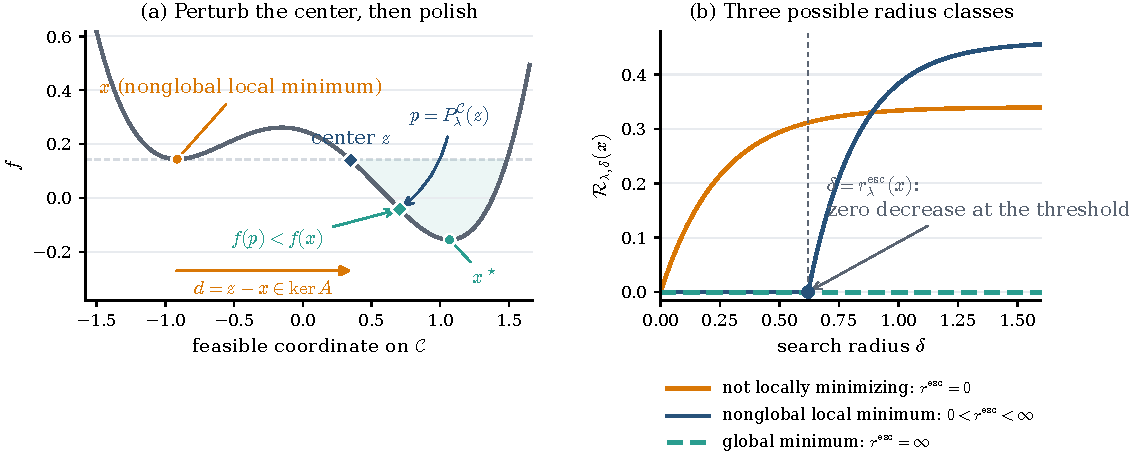
\includegraphics[width=0.98\textwidth]{figures/proximal_escape_schematic.pdf}
  \caption{Proximal-escape mechanism and radius classification.
  (a) A feasible center perturbation is followed by the safe constrained
  proximal map, producing the lower-value witness \(p\).
  (b) The three profiles in \Cref{thm:radius-classification}; the
  positive-radius profile meets zero continuously at its threshold.
  Panel~(b) is schematic.}
  \label{fig:proximal-escape-schematic}
\end{figure}

The direct decrease also induces a local feasible support curvature:
\begin{equation}
  \begin{aligned}
  \beta_r^{\Cset}(x)
  &:=
  \sup_{\substack{u\in\Cset\cap\dom f\\0<\norm{u-x}\le r}}
  \frac{2[f(x)-f(u)]_+}{\norm{u-x}^{2}}\\
  &=
  \inf\left\{
    \beta\ge0:
    x\in\argmin_{\substack{u\in\Cset\\\norm{u-x}\le r}}
       \left(f(u)+\frac{\beta}{2}\norm{u-x}^{2}\right)
  \right\},
  \end{aligned}
  \label{eq:local-support-threshold}
\end{equation}
where both expressions take values in \([0,+\infty]\).  The supremum of an
empty set is zero; if the quotient is unbounded, the admissible set in the
infimum representation is empty and \(\inf\varnothing=+\infty\).  In
particular,
\(\beta_r^{\Cset}(x)=0\) if and only if
\(\mathcal{S}_r(x)=0\).  The multiplier-free quantity
\(\beta_r^{\Cset}(x)\) describes feasible descent in a fixed ball.  If
\(\beta_r^{\Cset}(x)>0\), then
\(\mathcal{S}_r(x)>0\), and \cref{eq:prox-dominates-direct} implies
\(r_{\lambda}^{\mathrm{esc}}(x)\le r\).  The local feasible quantity
\(\beta_r^{\Cset}(x)\) is distinct from the all-space Lagrangian threshold
\(\beta_{\crit}(x,y)\) in \cref{eq:beta-crit}.

\subsection{An envelope formulation}

\subsubsection{Three ordered decrease measures}

The map
\(d\mapsto f(P_\lambda^{\Cset}(x+d))\) defining
\cref{eq:escape-profile} need not be smooth, even though the safe proximal
map is single valued.  A smooth outer objective is obtained from the
constrained Moreau envelope:
\begin{equation}
  \mathcal{R}^{E}_{\lambda,\delta}(x)
  :=
  f(x)
  -\inf_{\substack{d\in\Tspace\\\norm d\le\delta}}
      \Moreau_\lambda^{\Cset}(x+d).
  \label{eq:envelope-drop}
\end{equation}
Together with the direct and polished decreases, this gives three measures
of improvement whose order determines the strength of their associated
rejection tests.

\begin{lemma}[Ordering of the three decrease measures]
  \label{lem:drop-order}
  For every feasible \(x\) and every \(\delta\ge0\),
  \begin{equation}
    \mathcal{S}_\delta(x)
    \le
    \mathcal{R}^{E}_{\lambda,\delta}(x)
    \le
    \Rprox_{\lambda,\delta}(x).
    \label{eq:drop-order}
  \end{equation}
\end{lemma}

\begin{proof}
  For a feasible center \(z=x+d\), using \(u=z\) as a competitor gives
  \(\Moreau_\lambda^{\Cset}(z)\le f(z)\).  If
  \(p=P_\lambda^{\Cset}(z)\), then
  \[
    f(p)
    =
    \Moreau_\lambda^{\Cset}(z)
    -\frac{1}{2\lambda}\norm{p-z}^{2}
    \le\Moreau_\lambda^{\Cset}(z).
  \]
  Taking infima over the same tangent ball and subtracting from \(f(x)\)
  reverses both inequalities.
\end{proof}

The second inequality in \cref{eq:drop-order} makes every
\(\mathcal{R}^{E}_{\lambda,\delta}(x)>0\) a valid rejection certificate.  The
same proximal point also gives
\begin{equation}
  \nabla\Moreau_\lambda^{\Cset}(z)
  =
  \frac{1}{\lambda}
  \left(z-P_\lambda^{\Cset}(z)\right),
  \qquad
  f(P_\lambda^{\Cset}(z))
  =
  \Moreau_\lambda^{\Cset}(z)
  -\frac{\lambda}{2}
       \norm{\nabla\Moreau_\lambda^{\Cset}(z)}^{2}.
  \label{eq:recovery-identity}
\end{equation}
The polished value is available at no additional inner-prox cost.

Each decrease induces a corresponding infimal positivity radius:
\[
  r_{\lambda}^{P}(x)
  :=\inf\{\delta>0:\Rprox_{\lambda,\delta}(x)>0\},\quad
  r_{\lambda}^{E}(x)
  :=\inf\{\delta>0:\mathcal{R}^{E}_{\lambda,\delta}(x)>0\},
\]
\[
  r^{D}(x)
  :=\inf\{\delta>0:\mathcal{S}_{\delta}(x)>0\}.
\]
All three definitions use the convention \(\inf\varnothing=+\infty\).
The nesting in \cref{eq:drop-order} implies
\begin{equation}
  r_{\lambda}^{P}(x)
  \le r_{\lambda}^{E}(x)
  \le r^{D}(x),
  \qquad
  r_{\lambda}^{P}(x)=r_{\lambda}^{\mathrm{esc}}(x).
  \label{eq:radius-order}
\end{equation}
The smooth envelope can detect an escape no earlier than exact proximal
polishing and no later than a search restricted to the perturbed center.
For a proximal fixed point \(x\), this comparison has a complementary
lower bound:
\begin{equation}
  (1-\lambda\rho)r^D(x)
  \le r_\lambda^P(x)\le r_\lambda^E(x)\le r^D(x).
  \label{eq:radius-scale-bound}
\end{equation}
Indeed, let \(\mathcal L_x=\{u\in\Cset:f(u)<f(x)\}\), so that
\(r^D(x)=\dist(x,\mathcal L_x)\).  Any polished escape
\(p=P_\lambda^{\Cset}(x+d)\in\mathcal L_x\) satisfies
\[
  r^D(x)\le\norm{p-x}
  \le\frac{\norm d}{1-\lambda\rho}.
\]
Taking the infimum over such perturbations proves the lower bound.  If
\(\mathcal L_x\) is empty, all four quantities in
\cref{eq:radius-scale-bound} are infinite.  Polishing therefore changes
the center-space scale needed to discover decrease, not the underlying
optimality classification.

\subsubsection{A single-level representation}

Interchanging the outer-center and inner-proximal minimizations yields the
following single-level representation.
\begin{lemma}[Soft-ball representation]
  \label{lem:soft-ball}
  For every feasible \(x\) and every \(\delta\ge0\),
  \begin{equation}
    \inf_{\substack{d\in\Tspace\\\norm d\le\delta}}
      \Moreau_\lambda^{\Cset}(x+d)
    =
    \inf_{u\in\Cset}
    \left\{
      f(u)
      +\frac{(\norm{u-x}-\delta)_+^{2}}{2\lambda}
    \right\}.
    \label{eq:soft-ball}
  \end{equation}
\end{lemma}

\begin{proof}
  Expanding the envelope and interchanging two infima gives
  \[
    \inf_{\substack{u\in\Cset,\ d\in\Tspace\\\norm d\le\delta}}
    \left\{
      f(u)+\frac{1}{2\lambda}\norm{u-x-d}^{2}
    \right\}.
  \]
  Since \(u-x\in\Tspace\), the distance from \(u-x\) to the tangent ball
  \(B_\delta(0)\cap\Tspace\) is
  \((\norm{u-x}-\delta)_+\).  Minimizing first in \(d\) proves
  \cref{eq:soft-ball}.
\end{proof}

Equation~\eqref{eq:soft-ball} shows that the envelope search replaces the
hard local ball in \cref{eq:direct-drop} by a quadratic penalty on distance
outside that ball.  The representation is exact, although the resulting
global outer problem remains generally nonconvex.

Evaluating this envelope requires a constrained proximal point.  We first
describe two ways to obtain it, then combine these evaluations with a
projected search and a finite rejection test.
